\chapter{Аналитический раздел}

В данном разделе приводится классификация сетевых атак. 
Рассматривается технология нейронных сетей и принцип работы нейронных сетей. Описываются архитектуры нейронных сетей, их применение в задачах классификации. 
Проводится обзор существующих методов обнаружения сетевых атак.


\section{Анализ предметной области}

\textbf{Сетевая атака} \cite{second} --- это действие или последовательность связанных между собой действий, использующих уязвимости информационной системы и приводящих к нарушению политики безопасности. Под политикой безопасности подразумевается набор критериев и правил, описывающих информационные процессы в системе, выполнение которых обеспечивает необходимое условие безопасности системы.

\subsection{Модели атак}

\textbf{Классическая модель} атаки выстраивается по принципу  <<один к одному>>, как показано на рисунке 1.1, или <<один ко многим>>, как показано на рисунке 1.2. Для защиты от таких атак разработчики внедряют сенсоры системы защиты, передающие информацию на центральный аппарат управления.
Благодаря этому обеспечивается масштабируемость системы и простота удаленного управления. Однако такое решение не распространяется на модель с распределенными атаками \cite{third}.

\imgsvg{attack_model_1}{h!}{0.3}{12}{1}{Сетевая атака <<один к одному>>}
\clearpage
\imgsvg{attack_model_2}{h!}{0.5}{12}{1}{Сетевая атака <<один ко многим>>}


В \textbf{распределенной модели} используется принцип <<многие к одному>>, как показано на рисунке 1.3, или <<многие ко многим>>, как показано на рисунке 1.4. Данная атака осуществляется в два этапа. На первом этапе ищутся узлы сети, которые впоследствии задействуются для реализации распределенной атаки. Второй этап представляет собой посылку большого количества запросов на атакуемый сетевой узел.
Отправка запросов осу­ществляется с помощью скомпроме­тированных систем-посредников, на которых установлены специальные агенты, реализующие распределенную атаку. Агенты делятся на два типа: <<мастер>> и <<демон>>. Злоумышленник управляет небольшим числом <<мастеров>>, а те управляют <<демонами>>.
Стоит отметить, что блокирование одного или нескольких <<мастеров>> или <<демонов>> не приводит к завершению атаки \cite{third}.

\clearpage

\imgsvg{attack_model_3}{h!}{0.5}{12}{1}{Сетевая атака <<многие к одному>>}
\imgsvg{attack_model_4}{h!}{0.5}{12}{1}{Сетевая атака <<многие ко многим>>}

\subsection{Классификация сетевых атак}

Большинство сетевых атак нацелены на изменение определенных параметров безопасности системы. Например, с помощью некоторых атак злоумышленник может получить возможность просматривать передаваемые сообщения, но не изменять их. Другие атаки могут позволить злоумышленнику выполнить останов некоторых компонент системы, при этом не предоставляя доступ к ресурсам, хранящимся в данной системе \cite{third}.

Существует множество различных типов классификации атак. Например, деление на внешние и внутренние, пассивные и активные, умышленные и неумышленные.
Однако, все сетевые атаки можно разделить на два класса: пассивные и активные \cite{third}.

\textbf{Пассивная атака} \cite{fourth} --- это атака, при которой у злоумышленника нет доступа к модификации передаваемых сообщений и возможности добавления собственных сообщений в информационный канал между отправителем и получателем.
Основная цель пассивной атаки --- прослушивание передаваемых сообщений и анализ сетевого трафика.

\imgsvg{passive}{h!}{0.75}{12}{1}{Пассивная атака}

Одной из разновидностей пассивных атак являются \textbf{атаки сканирования} \cite{fifth}. 
Атаки сканирования не нацелены на проникновение в систему. Они помогают злоумышленнику определять:

\begin{itemize}
    \item топологию сети;
    \item активные хосты в сети;
	\item выполняемое на хостах ПО сервера;
	\item номера версий обнаруженного ПО.
\end{itemize}

Наиболее популярной атакой сканирования является \textbf{PortScan-атака (от англ. Port Scanning)}. 
Сканируя порты, злоумышленник пытается определить следующие параметры системы: открытые порты, базовую операционную систему,
поддерживаются ли неаутентифицированные входы в систему и т.д. Это выясняется путем отправки пакетов с флагами на
различные порты целевой системы, чтобы выяснить, является ли порт уязвимым и может ли он быть использован для
проникновения в систему.


% На рисунке 1.6 представлены инструментальные средства для осуществления атаки сканирования.

% \imgsvg{types}{h!}{0.8}{10}{1}{Инструментальные средства для осуществления атаки сканирования}



\textbf{Активная атака} \cite{six} --- это атака, при которой у злоумышленника имеется возможность модифицировать передаваемые сообщения и добавлять собственные. Существуют следующие виды активных атак:


\begin{enumerate}

    \item \textbf{Отказ в обслуживании --- DoS-атака (англ. Denial of Service)} \cite{fifth}. Отказ в обслуживании нарушает функционирование сетевых сервисов. Суть данной атаки заключается в следующем: на сетевой сервис поступает значительное количество запросов, в результате чего сетевой сервис перестает обрабатывать запросы реальных клиентов, а злоумышленник может перехватывать все сообщения направленные определенному адресату. DoS-атака базируется на классической модели атак. %\imgsvg{dos}{h!}{0.4}{10}{1}{DoS-атака}
    \item \textbf{Распределенный отказ в обслуживании --- DDoS-атака (от англ. Distributed Denial of Service)} \cite{fifth}. Основным отличием DDoS-атаки от DoS-атаки является использование распределенной модели атак.
    \item \textbf{DDoS Hulk (от англ. Distributed Denial of Service HTTP Unbearable Load King)} DDoS Hulk атака --- это тип DDoS-атак, который основывается на использовании HTTP протокола, для усиления и ускорения атаки. Нападающий использует несколько ботнетов для отправки огромного количества запросов на сервер, с целью перегрузить его и сделать недоступным для легитимных пользователей.
    \item \textbf{DDoS Heartbleed} атака является сочетанием двух типов кибератак: DDoS-атака и атака на уязвимость Heartbleed в OpenSSL-шифровании. DDoS-атака направлена на перегрузку сети огромным количеством запросов, что делает сервис недоступным для легитимных пользователей. В то же время, атака на уязвимость Heartbleed позволяет злоумышленникам получить доступ к чувствительным данным, хранящимся в памяти сервера, в том числе логинам, паролям, кредитным картам и другим конфиденциальным данным. Комбинированное использование этих двух методов позволяет киберпреступникам делать не только сервис недоступным, но и кражу конфиденциальных данных, что является очень опасным для пользователей и компаний.
    \item \textbf{DDoS Slowloris} атака --- это тип DDoS атаки, который основывается на отправке множества неполных запросов на сервер с помощью открытых соединений HTTP. Неполные запросы не закрываются, поэтому соединение остается открытым и приводит к выделению большого количества ресурсов сервера. Это приводит к замедлению, а в итоге и к отказу в обслуживании сервера или веб-сайта.
    \item \textbf{Атака полным перебором --- Brute Force } \cite{seventh}. Brute Force --- это атака с угадыванием паролей, учетных данных для входа в систему, ключей шифрования и прочей информации. Основная цель атаки полным перебором --- получить несанкционированный доступ к данным, системам или сетям.
    \item \textbf{Межсайтовый скриптинг --- XSS (от англ. Cross-Site Scripting)} \cite{sixtheen}. XSS --- тип атаки на веб-системы, заключающийся во внедрении в выдаваемую веб-системой страницу вредоносного кода (который будет выполнен на компьютере пользователя при открытии им этой страницы) и взаимодействии этого кода с веб-сервером злоумышленника. Специфика подобных атак заключается в том, что вредоносный код может использовать авторизацию пользователя в веб-системе для получения к ней расширенного доступа или для получения авторизационных данных пользователя. Вредоносный код может быть вставлен в страницу как через уязвимость в веб-сервере, так и через уязвимость на компьютере пользователя.
    \item \textbf{Внедрение SQL-кода --- SQLi (от англ. SQL injection)} \cite{sixtheen}. SQLi --- один из распространённых способов взлома сайтов и программ, работающих с базами данных, основанный на внедрении в запрос произвольного SQL-кода. Внедрение SQL, в зависимости от типа используемой СУБД и условий внедрения, может дать возможность атакующему выполнить произвольный запрос к базе данных (например, прочитать содержимое любых таблиц, удалить, изменить или добавить данные), получить возможность чтения и/или записи локальных файлов и выполнения произвольных команд на атакуемом сервере.
    % \item \textbf{Модификация потока данных --- MITM-атака (Men In The Middle)} \cite{six}. MITM-атака --- это атака, с помощью которой злоумышленник перехватывает связь между клиентом и сервисом. Позиционируя себя между законным клиентом и сервисом, злоумышленник может отключить шифрование и перехватить сообщения, отправляемые клиенту или сервису. Это позволяет злоумышленнику получать конфиденциальную информацию, такую как учетные данные и другую личную информацию.  \imgsvg{mitm}{h!}{0.4}{10}{1}{MITM-атака}
    % \item \textbf{Создание ложного потока (фальсификация)} \cite{seventh}. Фальсификация означает попытку одного субъекта выдать себя за другого. С помощью этой атаки злоумышленник может получить привилегии, которые не предусмотрены данной системой. Привилегия позволяет злоумышленнику в дальнейшем нарушить конфиденциальность, доступность или целостность сервиса.
    % \item \textbf{Атака повторного воспроизведения --- Replay-атака} \cite{seventh}. Атака повторного воспроизведения --- атака на систему аутентификации путём записи и последующего воспроизведения ранее посланных корректных сообщений или их частей. Для совершения данного вида атаки злоумышленник пользуется несовершенством системы аутентификации потока данных. Злоумышленник перехватывает несколько пакетов или команд приложения, изменяет их и воспроизводит с целью выполнения несанкционированных действий. 
\end{enumerate}


%\imgsvg{replay}{h!}{0.4}{10}{1}{Replay-атака}

\section{Классификация методов обнаружения сетевых атак}

% Для классификации способов обнаружения сетевых атак буду рассмотрены следующие методы: Цепи Маркова, Метод $\chi^2$, Метод среднеквадратических отклонений, Анализ распределений интенсивности передачи пакетов, Анализ временных рядов, Пороговый анализ.

% Общий алгоритм выявления сетевых атак описывается следующим образом: 

% \begin{enumerate}
%     \item Собирается весь сетевой трафик, представленный как набор сетевых пакетов.
%     \item Вычисляются признаковые атрибуты сетевого трафика и строится профиль активности пользователя.
%     \item Созданный набор признаковых атрибутов сравнивается с набором характеристик нормального поведения пользователя.
%     \item Если в результате получилось весомое расхождение сравниваемых атрибутов, то фиксируется сетевая атака. В противном случае происходит изменение параметров нормального поведения.
% \end{enumerate}

Распознавание и реагирование на подозрительную деятельность,
нацеленную на нарушение сетевых или вычислительных ресурсов организации,
называется обнаружением сетевых атак.
Эффективность этого процесса сильно зависит от применяемых методов анализа.
На сегодняшний день основными методами обнаружения сетевых атак являются методы статистического анализа,
методы на основе знаний и методы машинного обучения.


\subsection{Методы статистического анализа}
Для защиты системы используется подход, при котором для каждого субъекта определяется профиль,
а любое отклонение от него считается несанкционированной деятельностью. 
Статистические методы универсальны, так как не требуют знания о возможных атаках на систему.
Однако при их использовании могут возникнуть трудности, например, отсутствие возможности определить новые типы атак, которые не были включены в выборку данных, на основе которой обучается модель.



\subsection{Методы на основе знаний}
Данные методы широко используются и заключаются в формулировании информации об атаках в виде правил или сигнатур.
Сигнатуры являются шаблонами, описывающими определенную атаку.
Если происходящие действия совпадают с одной из сигнатур или срабатывает одно из правил,
то такие действия считаются несанкционированными. Такие методы
характеризуются практически полным отсутствием ложных тревог, 
однако для поддержания их актуальности необходимо постоянно обновлять базы данных атак. Методы не 
является устойчивым к модификациям атак и не могут автоматически адаптироваться.

\subsection{Методы машинного обучения}
% Необходимость в гибкой адаптивной системе защиты от сетевых атак, 
% непрерывно изменяющихся условий сетевой активности, требует разработки такой системы, 
% которая могла бы детально проанализировать значительный объем сетевого трафика на постоянно меняющихся условиях. 
% Нейронные сети являются альтернативой системам, основанным на правилах. В отличие от методов на основе знаний, 
% которые дают пользователю определенный ответ за счет соответствия характеристик атаки и заранее заложенных 
% характеристик в базе знаний, нейронная сеть проводит анализ информации и дает возможность оценить,
% соответствуют ли анализируемые данные характеристикам, которые она научена распознавать.

Машинное обучение является эффективной технологией для обнаружения сетевых атак. Данная технология использует алгоритмы и методы обработки большого количества данных и создания моделей, которые могут определять наличие аномальной активности в сети.

Для обнаружения сетевых атак с помощью машинного обучения необходимо собрать большой объем данных о поведении сети. 
Данные включают в себя информацию о трафике, времени и местоположении источника трафика и других факторах. 
Эта информация затем анализируется с помощью методов машинного обучения, которые могут отслеживать паттерны поведения и обнаруживать аномальные события.


Основными плюсами использования машинного обучения в задачах обнаружения
сетевых атак являются:

\begin{itemize}
    \item гибкость. Методы машинного обучения позволяют анализировать данные сетевого трафика в условиях искажения или неполноты;
    \item быстрая скорость обработки информации. Скорость обработки информации с помощью машинного обучения достаточна для реагирования в режиме реального времени на проводимые атаки до того, как в системе появятся непоправимые повреждения;
    \item возможность прогнозирования. Выходные данные в методах машинного обучения могут быть интерпретированы в форме вероятности. Это предоставляет возможность прогнозирования дальнейшего развития атаки.
    % \item Способность анализировать характеристики умышленных атак и идентифицировать элементы, которые не похожи на те, что наблюдались в сети при ее обучении. Нейронная сеть может быть обучена распознавать известные подозрительные события с высокой степенью точности, а также может использовать эти знания для идентификации атак, которые неточно соответствуют характеристикам предыдущих вторжений.
\end{itemize}


\section{Нейронные сети}

Направление исследований в области искусственного интеллекта,
называемое нейронными сетями, основано на том, чтобы воссоздать работу нервной системы человека. 
Одним из ключевых аспектов является способность обучаться и исправлять ошибки, что в конечном итоге позволяет 
имитировать работу человеческого мозга, хотя и достаточно грубо \cite{neuralnet}.

Нейронные сети состоят из слоев узлов: входных данных, скрытых и выходных данных. 
У каждого узла есть веса и пороговое значение. Если вывод узла превышает порог, он активируется и 
пересылает данные на следующий уровень. Если нет, данные не передаются.

На рисунке \ref{fig:neuralnet} представлена модель работы нейронной сети, где $x_i$ --- входные данные, а $Y_j$ --- выходные данные.

\begin{figure}[H]
	\centering
	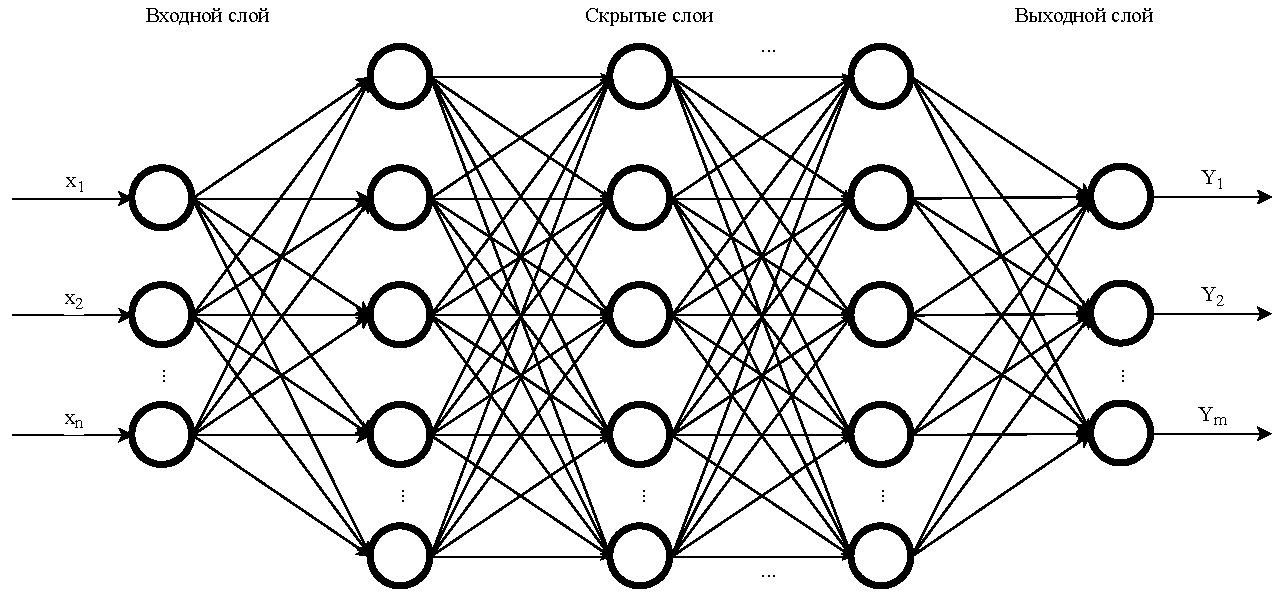
\includegraphics[width=\textwidth]{../img/neuralnet.pdf}
	\caption{Модель нейронной сети}
	\label{fig:neuralnet}
\end{figure}

\subsection{Принцип работы нейронных сетей}

Модель каждого отдельного узла нейронной сети может быть описана
как модель линейной регрессии \cite{linearreg} состоящая из входных данных, весовых коэффициентов, смещения (или порогового значения) и выходных данных.
Эту модель можно описать следующей формулой:

\begin{equation}
	\label{eq:nn0}
	\hat{y} = \sum_{i=1}^{m}w_ix_i + bias,
\end{equation}

\eqexplSetIntro{где}
\begin{eqexpl}[15mm]
\item{$\hat{y}$} прогнозируемое значение модели;
\item{$m$} количество факторов;
\item{$w$} весовой коэффициент фактора;
\item{$x$} единица входных данных;
\item{$bias$} значение ошибки.
\end{eqexpl}

Выходное значение для узла описывается по формуле:
\begin{equation}
	\label{eq:nn1}
	f(x_i) = \begin{cases}
		1 & \text{если $\hat{y} \ge 0$}\\
		0 & \text{иначе.}\\
		\end{cases}
\end{equation}


Необходимо назначить весовые коэффициенты после определения слоя входных данных. Они определяют важность каждого фактора: чем выше 
коэффициент, тем больший вклад данный фактор вносит в выходные данные.
Затем произведения входных данных и соответствующих им весовых коэффициентов суммируются.
Выходные данные передаются через функцию активации \ref{eq:nn1}, которая вычисляет результат. Если полученный результат превышает установленное пороговое значение,
узел срабатывает (активируется), передавая данные на следующий слой сети.

Для оценки точности модели необходимо использовать функцию стоимости (среднеквадратическая ошибка). Эта функция рассчитывается по формуле:

\begin{equation}
	\label{eq:nn3}
	Cost Function = \frac{1}{2m}\sum_{i=1}^{m}(\hat{y}-y)^2,
\end{equation}
\eqexplSetIntro{где}
\begin{eqexpl}[15mm]
	\item{$i$} индекс выборки;
	\item{$\hat{y}$} прогнозируемое значение;
	\item{$y$} фактическое значение;
	\item{$m$} число выборок.
\end{eqexpl}




Конечная цель --- минимизировать функцию стоимости, чтобы обеспечить корректность для каждого отдельно взятого наблюдения. 
Для достижения точки сходимости или локального минимума в модели используется функция стоимости и обучение с подкреплением, 
которые корректируют весовые коэффициенты и смещение. Алгоритм градиентного спуска позволяет определить стратегию уменьшения 
количества ошибок или минимизации функции стоимости. Каждый шаг обучения корректирует параметры модели, пока не будет достигнут 
минимум. Рисунок \ref*{fig:cost} показывает процесс минимизации функции стоимости.

\begin{figure}[H]
	\centering
	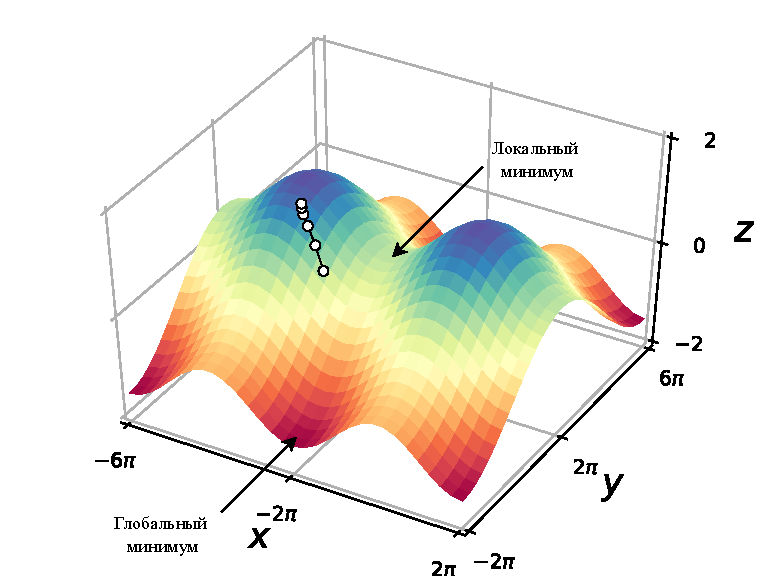
\includegraphics[width=\textwidth]{../img/cost.pdf}
	\caption{Минимизация функции стоимости}
	\label{fig:cost}
\end{figure}


\subsection{Архитектуры нейронных сетей}


\textbf{Многослойная нейронная сеть (от англ. multilayer perceptron, MLP)} --- это архитектура нейронной сети, состоящая из нескольких слоев нейронов, каждый из которых полностью связан со следующим слоем.
Нейроны в каждом слое получают на вход значения активации от всех нейронов предыдущего слоя, производят линейную комбинацию этих значений с определенными весами и применяют к результату функцию активации для получения своего выходного значения. Эта операция выполняется для каждого нейрона в каждом слое.
Такие сети обычно используются для задач классификации и регрессии, где входные данные имеют множество признаков.

\textbf{Сверточная нейронная сеть (от англ. Convolutional Neural Network, CNN)} используется для обработки и классификации изображений, видео и других пространственных данных. CNN состоит из нескольких слоев: сверточных, объединяющих, полносвязных и слоя выхода. Сверточные слои обрабатывают входные данные 
с помощью взвешивания и объединения признаков из различных частей изображения. Объединяющие слои уменьшают размерность 
данных, снижая число параметров и значительно ускоряя вычисления. Полносвязные слои связывают все объединенные признаки в выходной слой.
CNN активно применяется в многих областях, включая компьютерное зрение, робототехнику, автоматическое управление транспортом, медицину и другие.

\textbf{Рекуррентная нейронная сеть, (от англ. Recurrent neural network, RNN)} --- используется для обработки последовательностей данных, например, временных рядов, текстов и аудиофайлов. 
RNN имеет входной слой, скрытый слой и выходной слой. Скрытый слой в RNN имеет рекуррентные связи, которые позволяют сохранять информацию о предыдущих состояниях и использовать ее в следующих шагах.
Это позволяет RNN обрабатывать переменную длину последовательности данных и изучать контекст и зависимости между элементами последовательноси

\section{Постановка задачи}
Формально задача обнаружения сетевых атак с использованием многослойной нейронной сети может быть описана с помощью IDEF0-диаграммы, представленной на рисунке \ref*{img:idef}.

\imgs{idef}{H}{1}{Постановка заадчи}{}{}

\section{Применение машинного обучения в качестве классификатора сетевых атак}
Задача обнаружения сетевых атак сводится к задаче классификации сетевых атак. Процесс создания системы классификации сетевых атак схож с процессами создания других систем с применением машинного обучения:

\begin{enumerate}
    \item Необходимо собрать набор данных для обучения классификатора. Обучение модели нейронной сети для системы обнаружения сетевых атак будет производиться на наборе данных CICIDS2017.
    \item Каждую запись из обучающей коллекции нужно представить в виде вектора признаков.
    \item Для каждой записи нужно указать <<правильный ответ>>, т.е. тип сетевой атаки, по этим ответам и будет обучаться классификатор.
    \item Выбрать алгоритм классификации и обучить классификатор.
    \item Использовать полученную модель для обнаружения сетевых атак.
\end{enumerate}



\subsection{Метод опорных векторов}

SVM (от англ. Support vector machine) --- метод машинного обучения, применяемый в задачах классификации, основанный на построении гиперплоскости и ее анализе \cite{svm}.


Основной целью SVM как классификатора является поиск уравнения разделяющей гиперплоскости $w_1x_1+w_2x_2+…+w_nx_n+w_0=0$ в пространстве $R^n$, которая бы разделила два класса оптимальным образом. В формуле \ref{eq:nn6} представлен общий вид преобразования $F$ объекта $x$ в метку класса $Y$: 
\begin{equation}
	\label{eq:nn6}
	F(x) = sign(w^Tx-b).
\end{equation}

При рассмотрении обозначим $w = (w_1, w_2, …, w_n), b=-w_0$. Один из классов будет предсказываться для всех объектов, расположенных на одной стороне гиперплоскости, в то время как для объектов, находящихся на другой стороне, будет предсказываться другой класс.

В SVM веса $w$ и $b$ выбираются таким образом, чтобы объекты классов лежали как можно дальше от разделяющей гиперплоскости. 
Иначе говоря, алгоритм максимизирует зазор (англ. margin) между гиперплоскостью и объектами классов, которые расположены ближе всего к ней. Такие объекты называются опорными векторами.


На рисунке \ref{fig:svm1} изображен принцип работы метода.

\begin{figure}[H]
	\centering
	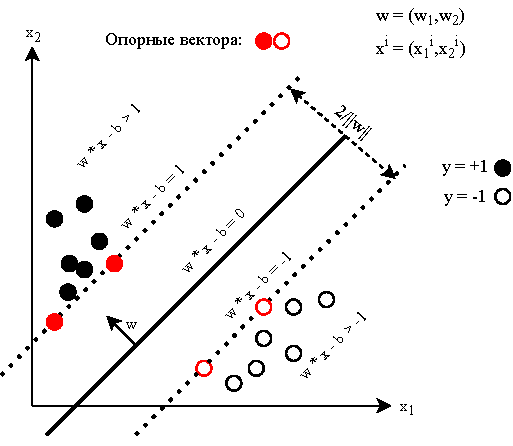
\includegraphics[width=\textwidth]{../img/svm1.pdf}
	\caption{Визуализация работы SVM}
	\label{fig:svm1}
\end{figure}

Здесь и далее скалярное произведение двух векторов будет обозначаться как $\langle a,b\rangle$ или $a^Tb$. Ширину разделяющий полосы будет показывать проекция вектора $w$, концами которого являются опорные вектора разных классов.

На рисунке \ref{fig:svm2} представлен вывод правил настройки весов.

\begin{figure}[H]
	\centering
	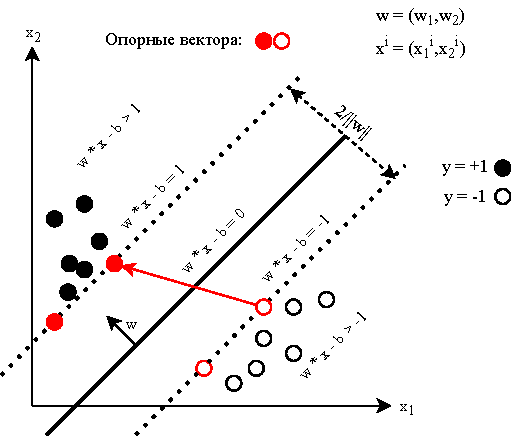
\includegraphics[width=\textwidth]{../img/svm2.pdf}
	\caption{Вывод правил настройки весов}
	\label{fig:svm2}
\end{figure}

В формулах \ref{eq:nn7} --- \ref{eq:nn10} представлен вывод правил настройки весов.

\begin{equation}
	\label{eq:nn7}
	\langle(x_+-x_-),\frac{w}{\Arrowvert w\Arrowvert}\rangle = \frac{\langle x_+,w\rangle - \langle x_-,w\rangle}{\Arrowvert w\Arrowvert} = \frac{(b+1)-(b-1)}{\Arrowvert w\Arrowvert} = \frac{2}{\Arrowvert w\Arrowvert},
\end{equation}

\begin{equation}
	\label{eq:nn8}
	\frac{2}{\Arrowvert w\Arrowvert} \rightarrow max,
\end{equation}

\begin{equation}
	\label{eq:nn9}
	\Arrowvert w\Arrowvert \rightarrow min,
\end{equation}

\begin{equation}
	\label{eq:nn10}
	\frac{w^Tw}{2} \rightarrow min.
\end{equation}

 Если $M > 1$, то объект $x$ классифицируется правильно, и находится на некотором удалении от разделяющей полосы. Алгоритм будет правильно классифицировать объекты, если выполняется условие, представленное в формуле \ref{eq:nn11}.
Величина $M=y(w^Tx-b)$ называется отступом объекта $x$ от границы классов. В случае отрицательного отступа алгоритм допускает ошибку на объекте. Если $M \in (0, 1)$,
то объект попадает внутрь разделяющей полосы. Если $M > 1$, то объект $x$ классифицируется корректно, и находится на удалении от разделяющей полосы. Алгоритм будет корректно классифицировать объекты, если выполняется условие, представленное в формуле \ref{eq:nn11}.

\begin{equation}
	\label{eq:nn11}
	y(w^Tx-b) \geq 1.
\end{equation}

\subsection{Алгоритм наивной Байесовской классификации}

Простой вероятностный классификатор, известный как наивный Байесовский классификатор, использует теорему Байеса с предположением о независимости \cite[]{twelve}.

Уравнение, описывающее взаимосвязь условных вероятностей статистических величин, известно как теорема Байеса. В байесовской классификации главный интерес заключается в определении вероятности отнесения к определенной категории по некоторым наблюдаемым характеристикам.

Целью классификации является поиск наилучшего класса, то есть имеющего наибольшую апостериорную вероятность $P(c_i|d_j)$:

\begin{equation}
	\label{eq:nn12}
    c^* = arg_{c_j \in C} maxP(c_i|d_j),
\end{equation}

где $d_i \in \Omega, c_j \in C$.

По формуле Байеса:

\begin{equation}
	\label{eq:nn13}
    P(c_i|d_j) = \frac{P(c_i)P(d_i|c_j)}{P(d_i)} \approx P(c_j)P(d_i|c_j), 
\end{equation}

где $P(c_j)$ --- априорная вероятность, что объект принадлежит $c_j$, а $P(d_i|c_j)$ --- вероятность встретить объект типа $d_i$ среди объектов класса $c_j$.

В прикладных приложениях для оценки параметров наивных Байесовских моделей часто применяется метод максимального правдоподобия, который позволяет работать с моделью, не обращая внимания на Байесовскую вероятность и байесовские методы.

Хотя классификатор имеет очень простые условия и наивный вид, он успешно справляется с обработкой самых разнообразных данных.

Достоинством наивного Байесовского классификатора является малое количество данных, необходимых для обучения, оценки параметров и классификации.



\subsection{Метод деревьев принятия решений}
Метод деревьев принятия решений --- машинное обучение, при котором
данные непрерывно разделяются в соответствии с определенным параметром \cite[]{classifiers}.

Дерево состоит из следующих элементов:

\begin{itemize}
    \item узлы --- сетевые параметры;
    \item листья --- метки классов;
    \item рёбра --- веса сетевых параметров.
\end{itemize}

Пример дерева принятия решения представлен на рисунке 1.12

\imgsvg{trees}{h!}{0.8}{10}{1}{Дерево принятия решений}

% TODO переписать
Процесс классификации заключается в поочередных перемещениях между
узлами дерева в зависимости от определенных признаков данного объекта.
Процесс классификации подходит к концу в тот момент, когда достигнут некий
конечный лист дерева. Лист, до которого дошел процесс классификации,
определяет определенный класс и, следовательно, рассматриваемый объект
является объектом данного класса. В задачах классификации чаще всего
встречаются бинарные деревья решений, и результат перехода по ребрам
определяется наличием или отсутствием некого признака в объекте.

% Лесом решений называют набор (ансамбль) из нескольких деревьев
% решений. С помощью комбинирования нескольких деревьев решений можно
% повысить качество классификации: решение о принадлежности объекта какому-либо классу принимается по большинству результатов, полученных у деревьев
% решений по отдельности.

% TODO переписать
Одним из главных преимуществ такого метода классификации является
легкость в интерпретации результата, а также меньший объем фильтрации.
Однако деревья решений имеют неустойчивый характер предсказаний, то есть
небольшое изменение входных данных влечет за собой значительное изменение
структуры дерева.


% \subsection{Метод логистической регрессии}
% % TODO переписать
% Логистическая регрессия является методом построения линейного
% классификатора, которая позволяет оценить апостериорные вероятности
% принадлежности объектов классам. Данный метод преобразовывает входные
% данные, используя логистическую сигмоидальную функцию, и возвращает
% значение вероятности принадлежности исследуемого объекта к одному из
% классов. Значение логистической регрессии всегда находится в промежутке от 0
% до 1, так как данный алгоритм основан на концепции вероятности.


% Логистическая регрессия бывает следующих типов:
% \begin{itemize}
%     \item бинарная – определяется, к какому из двух классов принадлежат исследуемые данные;
%     \item многолинейная – определяется принадлежность объекта к одному из нескольких классов, количество которых превышает 2.
% \end{itemize}

% Функцией, позволяющей сопоставить предсказанные моделью значения со
% значением вероятности, является сигмоидальная функция, представление
% которой приведено ниже на рисунке \ref*{fig:sigmoid}.

% \begin{figure}[H]
% 	\centering
% 	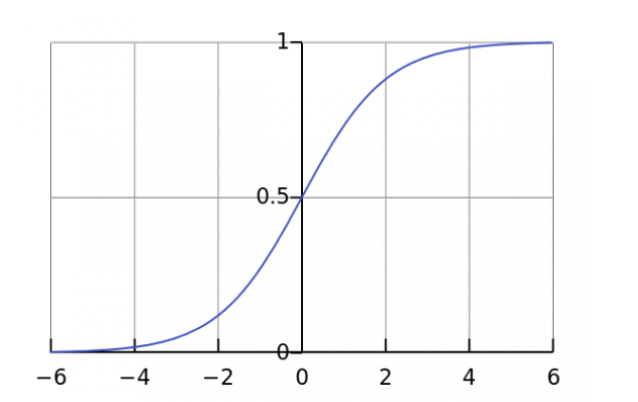
\includegraphics[width=100mm]{../img/sigmoid.png}
% 	\caption{Сигмоидальная функция}
% 	\label{fig:sigmoid}
% \end{figure}

% Формула сигмоидальной функции имеет вид:

% \begin{equation}
% 	\label{eq:nn14}
%     f(x) = \frac{1}{1 + e^{-x}}
% \end{equation}

% Также в алгоритме логистической регрессии используется функция,
% называемая функцией потерь, целью использования которой является
% минимизация значения ошибки классификации, позволяющая разработать более
% точную итоговую модель. Функция потерь для логистической функции выглядит
% следующим образом:

% \begin{equation}
% 	\label{eq:nn15}
% 	Cost(h_\theta(x), y) =  \begin{cases} -log(h_\theta(x)), & \mbox{если } y\mbox{ = 1} \\ -log(1 - h_\theta(x)), & \mbox{если } y\mbox{ = 0} \end{cases},
% \end{equation}
% где $h_\theta$ -- гипотеза логистической регрессии.

% При этом приведенные выше две функции можно представить в следующем виде:

% \begin{equation}
% 	\label{eq:nn16}
%     J(\theta) = -\frac{1}{m}\sum_{}^{}[y^{(i)}log(h_\theta(x(i))) + (1 - y^{(i)})log(1 - h_\theta(x(i)))]
% \end{equation}

% Для снижения значения функции потерь $J(\theta)$ используется градиентный
% спуск. Для достижения этого необходимо запустить функцию градиентного
% спуска для каждого параметра.

% \begin{equation}
% 	\label{eq:nn16}
%     \theta_j := \theta_j - \alpha \frac{d(J(\theta))}{d(\theta_j)}
% \end{equation}

% Вычисление будет производиться до тех пор, пока не будет достигнуто
% минимальное значение функции потерь.
% В качестве достоинств логистической регрессии можно отметить простоту
% реализации, а также легкость в обновлении модели для отражения новых данных.


% \subsection*{Пороговый анализ}

% В методе порогового анализа \cite{eight} сначала выбирается набор сетевых параметров, а именно:

% \begin{itemize}
%     \item IP-адреса источника и приемника --- \textbf{S/D};
%     \item тип и порт пакета --- \textbf{Tp};
%     \item длина пакета --- \textbf{L};
%     \item время фиксации пакета --- \textbf{Tm}.
% \end{itemize}

% Следовательное любое зафиксированное событие в сети можно описать вектором-объектом события $Tr = <S/D,  Tp, L, Tm>$.
% Далее из события $Tr$ извлекается объект $X = Tr<L>$, который соответствует длине зафиксированного пакета. Пусть $X_i$ --- событие из множества событий $X$, в некоторый момент времени. Тогда $Y_i$ --- аналогичный набор событий из множества, составляющего шаблон штатного функционирования сети. Затем выбирается коэффициент <<чувствительности>> $k = 0.8$. Тогда нижний порог определяется как $X_i > k Y_i$, а верхний как $X_i < \frac{Y_i}{k}$. После этого определяются краевые значения допустимых интервалов. Для этого берется выборочное среднее $\bar{X}$.

% \begin{equation}
%     \bar{X} = \frac{1}{n} \sum_{i = 0}^{n} X_i
% \end{equation}

% Допустимый диапазон определяется следующим неравенством: 

% \begin{equation}
%     \frac{\bar{X}}{2} < X_i <  \frac{3}{2} \bar{X}
% \end{equation}

% Нахождение вне рамок этого диапазона свидетельствует аномальному поведению.

% Недостатком данного метода является необходимость точного задания коэффициента <<чувствительности>> $k$ и отсутствие адаптивных механизмов для автоматического выбора порога \cite{fifthteen}.



% \subsection*{Анализ энтропии}

% Как известно энтропия множества $X$ определяется следующим образом: 

% \begin{equation}
%     H(X) = - \sum_{i = 1}^{n} p_i \log_2 p_i,
% \end{equation}

% где $p_i$ --- вероятность $i$-го состояния системы, $n$ --- количество всех возможных состояний системы \cite{fourteen}.

% Метод анализа энтропии \cite{nine} базируется на построении модели, которая максимизировала бы значение энтропии. Так как с увеличением количества уникальных записей происходит их равномерное распределение относительно классов множества $X$, что приводит к увеличению энтропии. 

% Для анализа энтропии выбирается следующий набор сетевых параметров 

% \begin{itemize}
%     \item IP-адрес источника;
%     \item IP-адрес приемника;
%     \item сетевой порт источника;
%     \item сетевой порт приемника.
% \end{itemize}

% \textbf{Алгоритм}

% \begin{enumerate}
%     \item Выбираются атрибуты для построения энтропийных временных рядов.
%     \item Строится множество временных рядов $T$.
%     \item Для каждого $T_i$ определяется ошибка прогноза на момент времени $t$: 
    
%     \begin{equation}
%         \delta_i = | Pred(T_i(t)) - T_i(t) |.
%     \end{equation}
    
%     \item Нормализуются  ошибки предсказания относительно дисперсии соответствующих временных рядов путем умножения на весовой коэффициент. Весовой коэффициент вычисляется по следующей формуле:
    
%     \begin{equation}
%         \omega_i = \frac{1}{\sigma_i} max(\sigma_1,...,\sigma_n).
%     \end{equation}

%     \item Вводится совокупная характеристика AS (anomaly score):
%     \begin{equation}
%         AS = \sum_{i = 1}^{n} \delta_i \omega_i
%     \end{equation}

%     \item Если $AS > AS_{thr}$, то фиксируется некая аномалия сетевого трафика. Пороговая величина $AS_{thr}$ определяется эмпирически в зависимости от количества базовых временных рядов $n$.
% \end{enumerate}


% \subsection*{Байесовский метод}

% Байесовская сеть \cite{ten} представляет собой модель, которая кодирует вероятностные отношения между некоторыми событиями и предоставляет механизм для вычисления условных вероятностей их наступления. В данном методе используются оценочные функции для определения вероятностей новых сетевых атак. Вследствие свойств предложенного метода системе не нужны предварительные знания о шаблонах атак.

% \textbf{Алгоритм}

% На первом этапе собирается информация о сетевых параметрах, а именно: 

% \begin{itemize}
%     \item IP-адрес источника;
%     \item IP-адрес приемника;
%     \item сетевой порт источника;
%     \item сетевой порт приемника;
%     \item состояние соединения;
%     \item временная метка.
% \end{itemize}

% Далее применяются правила ассоциации $X -> Y$ к записям соединений, где $X$ и $Y$ предусловие и постусловие правил, описанных внутри ядра системы соответственно. 
% Затем строятся профили нормального поведения клиентов системы и генерируются правила ассоциации, используемые впоследствии для обучения.

% Основным преимуществом данного метода является работа в режиме реального времени.


% \subsection*{SVM-метод}

% Метод опорных векторов --- SVM-метод (Support Vector Machine) \cite{eleven} рассматривается как один из ключевых методов обнаружения вторжений. 
% SVM является производным от линейно разделяемой гиперплоскости оптимальной классификации, и его основная идея может быть объяснена двумерным случаем представленным на рисунке 2.1.
% Существует обучающий набор $D = {(X_1, y_1), (X_2, y_2),...,(X_n, y_n)}$, где $X_i$ --- характеристический вектор обучающей выборке и $y_i$ --- соответствующая метка класса. $y_i$ принимает значения $+1$ или $-1$, указывая, принадлежит вектор к этому классу или нет. Говорят, что он линейно разделим, если существует линейная функция, которая может полностью разделить на два класса. В противном случае он нелинейно разделим.

% Рисунок 2.1 представляет собой линейно разделяемый случай, поскольку можно провести прямую линию, чтобы отделить вектор класса $+1$ от вектора класса $-1$.
% Существует бесчисленное множество таких линий, и так называемая оптимальная линия классификации требующая, чтобы две выборки были правильно разделены и чтобы интервал разделения был наибольшим. SVM завершает классификацию выборки путем поиска той, которая имеет наибольший интервал классификации.

% \imgsvg{svm}{h!}{0.8}{10}{1}{SVM-метод}

% Оптимальная линия классификации может быть выражена уравнением $\omega x + b = 0 \space (\omega \in R^n, b \in R)$, $\omega$ представляет собой вектор веса, а $b$ --- скаляр, называемый смещением. Точки над разделяющей гиперплоскостью удовлетворяются следующим образом:

% \begin{equation}
%     \omega x + b > 0.
% \end{equation}

% Аналогично, точки ниже разделяющей гиперплоскости удовлетворяются следующим образом:

% \begin{equation}
%     \omega x + b < 0.
% \end{equation}

% Мы можем отрегулировать вес, чтобы крайняя сторона гиперплоскости могла быть выражена как:

% \begin{equation}
%     \begin{split}
%     H1 : \omega x + b \ge 1, для y_i = 1; \\
%     H2 : \omega x + b \le 1, для y_i = -1.
%     \end{split}
% \end{equation}

% Это означает, что векторы, падающие на или выше $H1$, принадлежат классу $+1$, а векторы, падающие на или ниже $H2$, принадлежат классу $-1$.

% Обнаружение сетевой атаки эквивалентно задаче с двумя классификациями. Сначала собираются данные сетевого подключения для обучения, затем находится оптимальная классификационная гиперплоскость между данными нормального поведения и данными сетевой атаки \cite{thirteen}.

\subsection{Метод обратного распространения ошибки для обучения нейронных сетей}
Метод обратного распространения ошибки (от англ. backpropagation, BP) --- метод вычисления градиента, который используется при обновлении весов в многослойной нейронной сети \cite[]{eight}.

Идея BP состоит в распространении сигналов ошибки от выходов
многослойной нейронной сети к ее входам, в направлении, обратном прямому распространению сигналов в обычном режиме работы.

\begin{itemize}
    \item на вход нейрона поступает кортеж чисел вида $(x^1,...,x^n) \in \mathbb{R}^n$,
    \item на выходе нейрон выдает число $a = \sigma(\langle x, w \rangle - w_0)$, где $\sigma$ --- функция активации.
\end{itemize}

При заданной совокупности $w$ значений весовых коэффициентов $w_{ij}$ многослойная нейронная сеть определяет функцию $a_w$, 
отображающую каждый входной вектор $x \in \mathbb{R}^M$. Если задана обучающая выборка $S \subseteq \mathbb{R}^n \times \mathbb{R}^M$, 
то ошибкой на паре $(x, y) \in S$ называется число

\begin{equation}
	\label{eq:nn30}
	Q(x, y, w) = \frac{1}{2}(a_w(x)-y)^2.
\end{equation}

Задача алгоритма BP заключается в нахождении такой совокупности $w$ весовых коэффициентов, которые делают ошибки (\ref*{eq:nn3}) как можно меньше. Алгоритм BP решает эту задачу путем
выполнения нескольких итераций, каждая из которых состоит из двух частей:

\begin{itemize}
    \item выбор пары $(x, y) \in S$,
    \item нахождение ошибки \ref*{eq:nn30} на выбранной паре $(x, y)$ при текущем наборе весовых коэффициентов $w$ путем вычисления в <<прямом направлении>> выходов всех нейронов,
    \item коррекция весовых коэффициентов $w_{ij}$ путем вычисления в <<обратном направлении>> (сначала корректируются весовые коэффициенты последнего слоя, затем --- предпоследнего, и т.д.).
\end{itemize}

Алгоритм BP имеет следующий вид:

\begin{enumerate}
    \item Инициализация весов небольшими случайными значениями.
    \item Производятся итерации (до тех пор пока $Q$ не стабилизируется), каждая итерация заключается в вычислении по текущему набору $w$ весовых коэффициентов нового набора $w'$, который будет текущим в следующей итерации, и имеет следующий вид:
    \begin{itemize}
        \item случайно выбираются $(x,y) \in S, x = (x^1,...,x^n),y = (y^1,...,y^M)$,
        \item прямой выход: вычисляются выходы нейронов, и 
        \begin{equation}
            \begin{aligned}
                Q(x, y, w) = \frac{1}{2}\sum_{m=1}^{M}(a^m-y^m)^2\\
                \forall m = 1,...,M \quad \frac{\partial Q}{\partial a^m} = a^m - y^m = \xi^m,    
            \end{aligned}
            \label{eq:nn31}
        \end{equation}
        \item обратный ход (модификация весов в направлении $-\triangledown$):
        \begin{equation}
            \begin{aligned}                
                w'_{hm} = w_{hm} - \frac{\partial Q}{\partial w_{hm}}\eta,\\
                w'_{jh} = w'_{jh} - \frac{\partial Q}{\partial w_{jh}}\eta
            \end{aligned}
            \label{eq:nn32}
        \end{equation}
        где $\eta \in (0, 1)$ --- подбираемый параметр (темп обучения), и частные производные $\frac{\partial Q}{\partial w_{hm}}$, $\frac{\partial Q}{\partial w_{jh}}$ вычисляются следующим образом:
        пусть $u^1,...,u^H$ --- выходы первого слоя, тогда $\forall m = 1,...,M \quad \forall h = 1,...,H, \quad \forall j = 1,...n,$
        % \begin{equation}
            \begin{gather*}                
                a^m = \sigma(\sum_{h=1}^{H}w_{hm}u^h-w_{0m}),\\
                \frac{\partial Q}{\partial w_{hm}} = \frac{\partial Q}{\partial a^m}\frac{\partial a^m}{\partial w_{hm}} = \xi^m \sigma'(\sum_{h=1}^{H}w_{hm}u^h - w_{0m})u^h= \xi^m a^m (1 - a^m) u^h,\\
                \frac{\partial Q}{\partial w_{0m}} = \frac{\partial Q}{\partial a^m}\frac{\partial a^m}{\partial w_{0m}} = \xi^m \sigma'(\sum_{h=1}^{H}w_{hm}u^h - w_{0m})(-1)= -\xi^m a^m (1 - a^m),\\
                u^h = \sigma(\sum_{j=1}^{n}w_{jh} x^j - w_{0h}),\\
                \frac{\partial Q}{\partial u^h} = \sum_{m=1}^{M} \frac{\partial Q}{\partial a^m}\frac{\partial a^m}{\partial u^h} = \sum_{m=1}^{M} \xi^m \sigma'(\sum_{h=1}^{H}w_{hm}u^h - w_{0m})w_{hm}=\\
                =\sum_{m=1}^{M}\xi^m a^m (1 - a^m) w_{hm} = \zeta^h\\
                \frac{\partial Q}{\partial w_{jh}} = \frac{\partial Q}{\partial u^h}\frac{\partial u^h}{\partial w_{jh}} = \zeta^h \sigma'(\sum_{j=1}^{n}w_{jh}x^j - w_{0h}) x^j= \zeta^h u^h (1 - u^h)x^j,\\
                \frac{\partial Q}{\partial w_{0h}} = \frac{\partial Q}{\partial u^h}\frac{\partial u^h}{\partial w_{0h}} = \zeta^h \sigma'(\sum_{j=1}^{n}w_{jh}x^j - w_{0h})(-1)= -\zeta^h u^h (1 - u^h)
            \end{gather*}
            % \label{eq:nn33}
        % \end{equation}
    \end{itemize}

    Основным преимуществом является универсальность, поскольку данный метод работает с любой конфигурацией многослойной нейронной сети.
    К недостаткам можно отнести долгий процесс обучения, а также вероятность получить большие значения весов. Это может привести к
    тому, что большинство нейронов будут функционировать при очень больших значениях весовых коэффициентов, в области, где производная функции активации очень мала. Так как обратно распространяемая в процессе обучения ошибка пропорциональна этой 
    производной, то процесс обучения может стать парализованным.
\end{enumerate}

\subsection{Метод k-ближайших соседей}
Пусть задана обучающая выборка $S \subseteq X \times Y$ \cite[]{twelve}.
Если на множестве $X$ объектов задана метрика $p$, то $\forall x \in X$ объекты из множества $X_s$ можно упорядочить в соответствии с их близостью к $x$, т.е. расположить в последовательность

\begin{equation}
	\label{eq:nn34}
    x_1,...,x_{|S|},
\end{equation}
удовлетворяющую условию:
\begin{equation}
	\label{eq:nn35}
    p(x,x_1)\leq ... \leq p(x,x_{|S|})
\end{equation}

т.е. первым в \ref*{eq:nn34} расположен ближайший к $x$ объект, затем --- следующий по близости к $x$ объект, и т.д. $\forall i = 1,...,l$ объект $x_i$ из последовательности \ref*{eq:nn35} называется $i$–м ближайшим соседом к $x$.
Метод ближайших соседей для построения аппроксимирующей функции $a_S$ заключается в том, что выбираются 
\begin{itemize}
    \item натуральное число $k \geq 1 $ (число ближайших к $x$ объектов, ответы на которых учитываются при вычислении ответа $a_S(x)$),
    \item действительные числа $w_1 \geq ... \geq w_k > 0$, которые имеют смысл весов, определяющих вклад ближайших $k$ соседей объекта $x$ из обучающей выборки $S$ в вычисление ответа для объекта $x$, например,
    \begin{equation}
        \label{eq:nn36}
        \forall i = 1,...,k \quad w_i = \frac{k + 1 - i}{k}.
    \end{equation}
\end{itemize}
$\forall x \in X$ значение $a_S(x)$ определяется как такой ответ $y \in Y$, который максимизирует значение выражения
\begin{equation}
    \label{eq:nn37}
    \sum_{i=1}^{k}(y_{x_i}=y)w_i,
\end{equation}
т.е. как такой ответ $y$, который наиболее характерен среди ответов на $k$ ближайших соседей $x$ из обучающей выборки $S$.
Оптимальным является такое $k$, которое минимизирует риск
\begin{equation}
    \label{eq:nn38}
    \sum_{(x,y_x)\in S}^{}(a^k_{S \setminus \{(x,y_x)\}}(x) \ne y_x),
\end{equation}
где $a^k_S$ --- построенная аппроксимирующая функция в соответствии с приведенным выше определением.




\section{Сравнение рассмотренных методов}


Существуют различные способы оценки модели
классификации:

\begin{itemize}
    \item F-мера (f1-score);
    \item точность (precision);
    \item время обучения (training time);
    \item аккуратность (accuracy);
    \item полнота (recall).
\end{itemize}

\subsection{Аккуратность}
Наиболее простая метрика, определяющая долю
правильных ответов результатов модели. Рассчитывается следующим образом:
\begin{equation}
    \label{eq:nn39}
    accuracy = \frac{TP + TN}{TP + TN + FP + FN},
\end{equation}
где $TN$ --- истинно отрицательные ответы, $TP$ --- истинно положительные ответы,
$FN$ --- ложно отрицательные ответы, $FP$ --- ложно положительные ответы. 
Однако данная метрика не подходит в случае, если объем данных между
классами распределен неравномерно.

\subsection{Точность}
Данная метрика показывает долю правильных ответов относительно
всех положительных ответов в пределах одного класса. Формула вычисления приведена ниже:
\begin{equation}
    \label{eq:nn40}
    precision = \frac{TP}{TP + FP}.
\end{equation}
Учитывая данную метрику, можно сказать о количестве ложно
положительных предсказаний и сделать вывод о достаточности объема данных
других классов.

\subsection{Полнота}
Полнота --- это доля истинно положительных классификаций. С её
помощью можно сказать какую долю объектов, которые действительно
относятся к данному классу, модель предсказала верно.
\begin{equation}
    \label{eq:nn41}
    recall = \frac{TP}{TP + FN}.
\end{equation}
Полнота показывает способность алгоритма обнаруживать данный класс.

\subsection{F-мера}
F-мера --- это гармоническое среднее между точностью и полнотой. Данная
метрика позволяет найти баланс между этими метриками, так как на практике
зачастую невозможно достичь максимальной точности и полноты одновременно.

\begin{equation}
    \label{eq:nn42}
    F1 = \frac{2 \times precision \times recall}{precision + recall}
\end{equation}
Метрика достигает своего максимума при наибольших значениях полноты
и точности, и стремится к нулю, если один из аргументов близок к нулю.


% \subsection{Метод обратного распространения ошибки}

% Метод обратного распространения ошибки (от англ. backpropagation) --- метод вычисления градиента, который используется при обновлении весов в нейронной сети.

% Рассмотрим нейронную сеть без скрытых слоев (рисунок \ref{fig:simple}), с двумя входными вершинами и одной выходной, в которых каждый нейрон использует линейную функцию активации, которая является взвешенной суммой входных данных.




% Изначально веса задаются случайно. Затем, нейрон обучается с помощью тренировочного множества, которое состоит из множества троек $(x_1, x_2, \hat{y})$, где $x_1$ и $x_2$ --- это входные данные сети и $\hat{y}$ --- правильный ответ. Начальная сеть, приняв на вход $x_1$ и $x_2$, вычислит ответ $y$, который вероятно отличается от $\hat{y}$. Общепринятый метод вычисления несоответствия между ожидаемым $\hat{y}$ и получившимся $y$ ответом --- квадратичная функция потерь:
% \begin{equation}
% 	\label{eq:nn4}
% 	E = (\hat{y}-y)^2,
% \end{equation}
% \eqexplSetIntro{где}
% \begin{eqexpl}[15mm]
% 	\item{$E$} ошибка.
% \end{eqexpl}

% В качестве примера, обучим сеть на объекте $(1, 1, 0)$, таким образом, значения $x_1$ и $x_2$ равны 1, а $\hat{y}$ равно 0. Построим график зависимости ошибки $E$ от действительного ответа $y$, его результатом будет парабола (рисунок \ref{fig:error}).

% \begin{figure}[H]
% 	\centering
% 	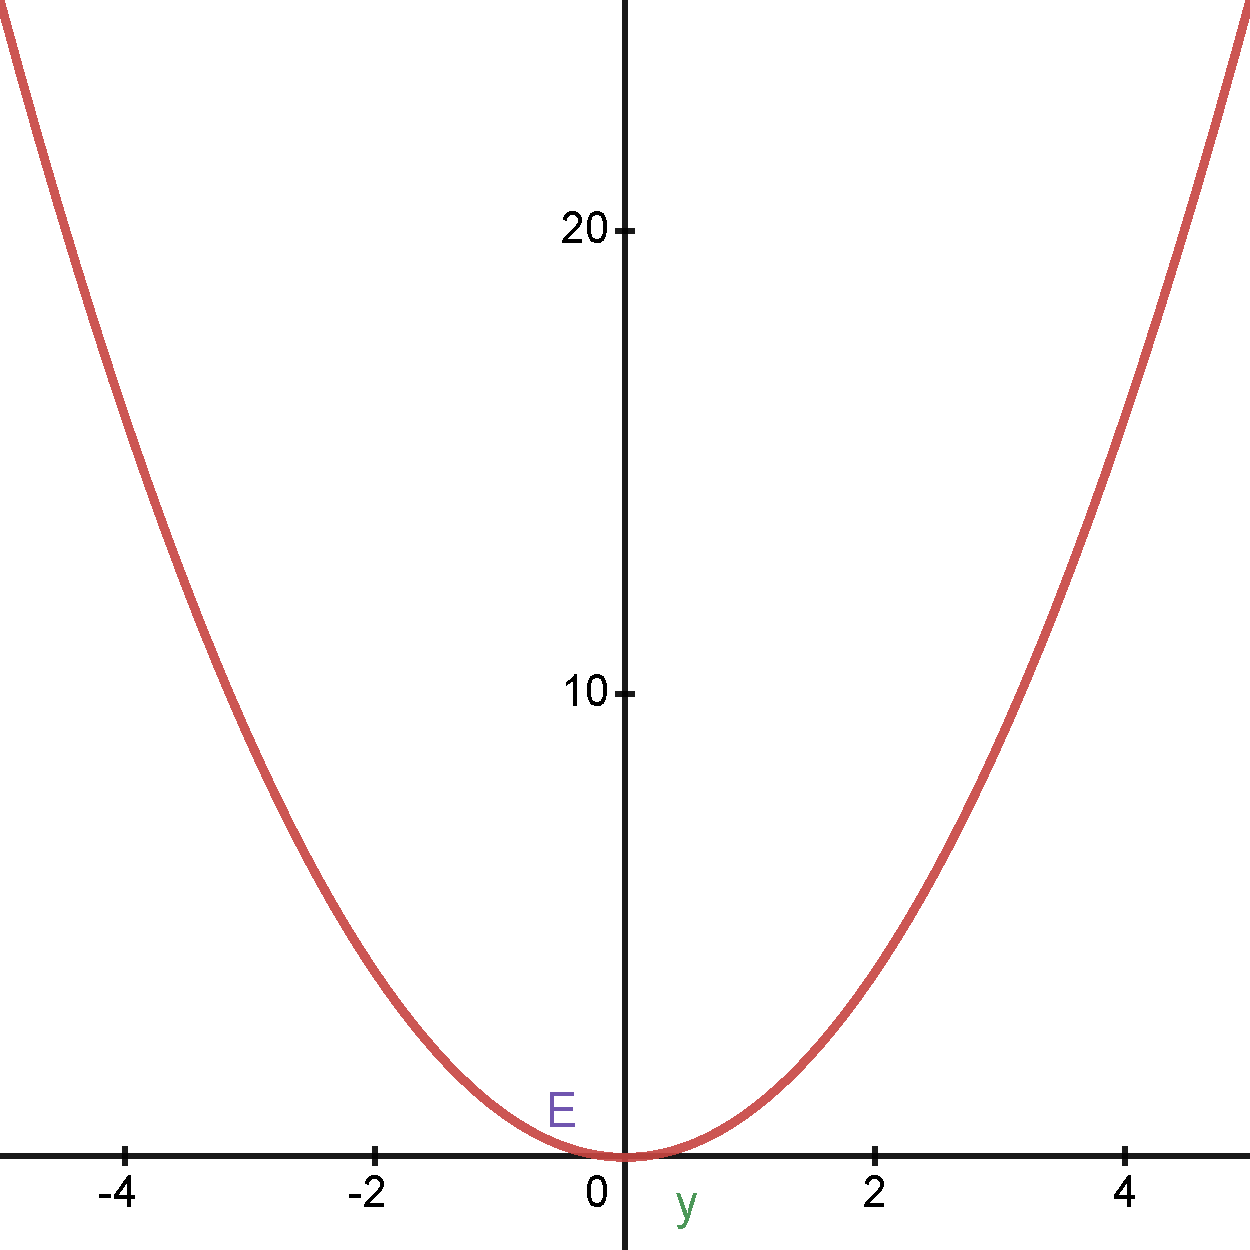
\includegraphics[width=80mm]{../img/error.pdf}
% 	\caption{Зависимость ошибки от действительного ответа}
% 	\label{fig:error}
% \end{figure}

% Минимум параболы соответствует ответу $y$, минимизирующему $E$. 
% Если тренировочный объект один, минимум касается горизонтальной оси, следовательно ошибка будет равна нулю и сеть выдаст ответ 
% $y$, равный ожидаемому ответу $\hat{y}$. А значит, задача преобразования входных значений в выходные сводится к 
% задаче поиска функции, результатом которой является минимальная ошибка.

% В таком случае, выходное значение нейрона --- взвешенная сумма всех его входных значений:
% \begin{equation}
% 	\label{eq:nn5}
% 	\hat{y} = x_1w_1 + x_2w_2,
% \end{equation}
% \eqexplSetIntro{где}
% \begin{eqexpl}[15mm]
% 	\item{$w_1, w_2$} веса на ребрах, соединяющих входные вершины с выходной.
% \end{eqexpl}

\subsection{Результаты сравнений}

Результаты сравнений на наборе данных UNSW-NB15 \cite{unsw} приведены в таблице \ref{tbl:compare}.

% Настройка выравнивание колонки по центру
\newcolumntype{P}[1]{>{\centering\arraybackslash}p{#1}}

\begin{center}
    \captionsetup{justification=raggedleft,singlelinecheck=off}
    \begin{longtable}[c]{|>{\small}P{3.5cm}|>{\small}P{1.5cm}|>{\small}P{3cm}|>{\small}P{2cm}|>{\small}P{1.9cm}|>{\small}P{1.8cm}|}
    \caption{Сравнение методов\label{tbl:compare}}
    \\ \hline
        & 
        \textbf{F-мера} &
        \textbf{Аккуратность} &
        \textbf{Точность} &
        \textbf{Полнота} &
        \textbf{Время} 
    \\ \hline
        \textbf{К-ближайших соседей} &
        0.96 &
        0.97 &
        0.96 &
        0.97 &
        Высокое
    \\ \hline
        \textbf{BP} &
        0.9 &
        0.92 &
        0.89 &
        0.92 &
        Среднее
    \\ \hline
        \textbf{Деревья принятия решений} &
        0.92 &
        0.9 &
        0.91 &
        0.93 &
        Низкое
    \\ \hline
        \textbf{SVM} &
        0.88 &
        0.9 &
        0.87 &
        0.88 &
        Среднее 
    \\ \hline
        \textbf{Наивная Байесовская классификация} &
        0.79 &
        0.8 &
        0.78 &
        0.78 &
        Низкое
    \\ \hline
\end{longtable}
\end{center}

\section{Вывод}

Были рассмотрены модели сетевых атак, а также была приведена их классификация.
Дано пределение понятия нейронной сети, описаны архитектуры нейронных сетей и принцип их работы.
Рассмотрены методы машинного обучения для решения задачи классификации сетевых атак.
В качестве выбранной технологии для разрабатываемого метода выбрана многослойная нейронная сеть, так как она широко используется в задачах классификации. Исходя из результатов сравнительного анализа для решения задачи классификации сетевых атак был выбран метод обратного распространения ошибки.


% @online{gs1-128,
%   language = "russian",
%   title    = "СТАНДАРТ ГС1 РУС [Электронный ресурс]",
%   note     = "URL: \url{https://www.gs1ru.org/wp-content/uploads/2017/02/СТО-30_V_1_открыт.pdf} (дата обращения: 20.11.2022)"
% }
